\maketitle
\tableofcontents
\newpage

\section{Zielsetzung}
Ziel dieses Versuches ist es, gedämpfte und erzwungene Schwingungen zu untersuchen.
\section{Theorie}
Ein Schwingkreis besteht in seiner einfachsten Form aus einem Kondensator mit der Kapzität
$C$ und einer Spule mit der Induktivität $L$. Die Energie in diesem Schwingkreis oszilliert
zwischen den beiden Energiespeichern und hat als mögliche Maxima ein maximales magnetisches
Feld in der Spule und einen maximal aufgeladenen Kondensator. Falls ein idealer Draht
vorliegt, wird diese $\textbf{ungedämpfte Schwingung}$ für $t \to \infty$ unverändert schwingen.
\subsection{Gedämpfte Schwingung}
\begin{figure}
  \centering
  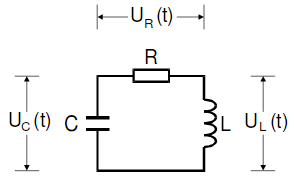
\includegraphics[scale=0.6]{gSchwingkreis.png}
  \caption{Schaltbild eines gedämpften Schwingkreises \cite{anleitung}.}
  \label{fig:1}
\end{figure}

Falls nun aber ein endlicher Widerstand $R$ in den Schaltkreis eingebaut wird, siehe \ref{fig:1},
dann wird ein Teil der elektrischen Energie an diesem ohmschen Widerstand in Wärme umgewandelt.
Damit fallen die Amplituden der Spannung und des Stromes mit der Zeit ab und es entwickelt sich
eine $\textbf{gedämpften Schwingung}$. Das Gesetz zwischen der Absinken der Amplitude und der Zeit
lässt sich aus dem zweiten Kirchhoffschen Gesetz, mit den Spannungen aus Abbildung \ref{fig:1},
herleiten
\begin{equation}
    U_R (t) + U_L (t) + U_C (t) = 0 \, .
    \label{eqn:1}
\end{equation}
Daraus entwickelt man eine lineare homogene Differentialgleichung 2. Ordnung der Form
\begin{equation}
    \frac{\symup{d^2} I}{\symup{d^2}t} + \frac{R}{L} \frac{\symup d I}{\symup d t} +
    \frac{1}{LC} \, I = 0 \, ,
    \label{eqn:2}
    %Hier eventuell eher zwei Punkte als Ableitung
\end{equation}
welche als Lösung
\begin{equation}
  I'(t) = e^{-2 \pi \mu t} \left(A e^{i 2 \pi \nu t} + B e^{-i 2 \pi \nu t}\right)
  \label{eqn:3}
\end{equation}
mit $A$ und $B$ als beliebige Zahlen aus $\mathbb{C}$ und den Abkürzungen
\begin{equation*}
    \begin{split}
        2 \pi \mu = \frac{R}{2L} \\
        2 \pi \nu = \sqrt{\frac{1}{LC} - \frac{R^2}{4L^2}}
    \end{split}
\end{equation*}
besitzt. Für den weiteren Verlauf ist es erforderlich zu ermitteln, ob $\nu$
reell oder imaginär ist. Deshalb wird eine Fallunterscheidung ausgeführt:
\begin{itemize}
  \item $\nu$ ist reell:

    Damit in diesem Fall $I'(t)$ reell wird, muss $A = \overline{B}$ gelten. Mit
    geeigneten Ansätzen erhält man schließlich
    \begin{equation}
        I(t) = A_0 \, e^{-2 \pi \mu t} \, \symup{cos} \left(2 \pi f t + \eta \right)
        \label{eqn:4}
    \end{equation}
    mit $A_0$ und $\eta$ als beliebige Zahlen aus $\mathbb{R}$ und $f$ als Frequenz der
    Schwingung. Gleichung \eqref{eqn:4} stellt eine Schwingungsgleichung für eine
    $\textbf{gedämpfte Schwingung}$ dar, deren Amplitude offensichtlich exponentiell gegen 0 strebt.
    Für die Schwingungsdauer ergibt sich
    \begin{equation}
      T = \frac{1}{f} = \frac{2 \pi}{\sqrt{\frac{1}{LC} - \frac{R^2}{4L^2}}} \, .
      \label{eqn:5}
    \end{equation}
    Die Abnahmegeschwindigkeit steckt im Exponenten der e-Funktion in \eqref{eqn:4},
    nämlich im $\mu$. Daraus lässt sich die Abklingdauer $T_\symup{ex}$ definieren
    \begin{equation}
        T_\symup{ex} = \frac{1}{2 \pi \mu} = \frac{2L}{R} \, .
        \label{eqn:6}
    \end{equation}
  \item $\nu$ ist imaginär:

    Gleichung \eqref{eqn:3} besteht nur noch aus vollständig reellen Exponentialfunktionen,
    sodass \eqref{eqn:4} keinen oszillatorischen Anteil besitzt. Dies nennt man
    aperiodische Dämpfung. Abhängig von $A$ und $B$ strebt $I(t)$ monoton gegen 0 oder
    erreicht noch einen Extremwert. Für das Experiment von Bedeutung ist der Spezialfall
    \begin{equation}
        \frac{1}{LC} = \frac{R_{\symup{ap}}^2}{4L^2} \, ,
        \label{eqn:7}
    \end{equation}
    der $\textbf{aperiodischer Grenzfall}$ heißt und für den $f = 0$ ist. Die Amplitude des Stroms strebt maximal schnell
    gegen 0 und besitzt keinen Überschwinger.
\end{itemize}
\subsection{Erzwungene Schwingung}
\begin{figure}
  \centering
  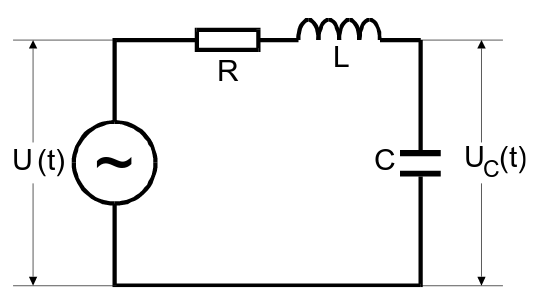
\includegraphics[scale=0.4]{eSchwingkreis.png}
  \caption{Schaltbild einer erzwungenen Schwingung.}
  \label{fig:2}
\end{figure}

\section{Durchführung}

\subsection{Versuchsaufbau}

\subsection{Versuchsdurchführung}
\section{Auswertung}

\section{Diskussion}
\newpage
\nocite{*}
\printbibliography
